\section{Introduction}

This is a simple template for a brief report in a seminar. If you have
used \LaTeX{} before, you should have no trouble accustoming yourself to
it. You may use UTF-8 characters in the document, provided your font supports
them:
%
\begin{quote}
  Allein der Vortrag macht des Redners Glück
\end{quote}
%
The default font in this document supports~(at least) German, French,
and English characters. You should hence have no problem typesetting
complicated names such as \emph{Henri Poincaré} or \emph{Cédric
Villani}. In the following, this document discusses how to typeset
certain things.

\subsection{Typesetting tables}

Tables should be wrapped in a \verb|table| environment and have a proper
caption and label for references. Moreover, typographically correct
lines~(also known as \emph{rules}) should be used. The following example
demonstrates this:
%
\begin{center}
  \begin{verbatim}
    \begin{table}
      \centering
      \begin{tabular}{lSS}
        \toprule
        [...]
        \midrule
        Mount Everest & 8848 & 8848\\
        [...]
        \bottomrule
      \end{tabular}
    \end{table}
    \caption{%
      [...]
    }
    \label{tab:Mountains}
  \end{verbatim}
\end{center}
%
\autoref{tab:Mountains} on \autopageref{tab:Mountains} shows how this
looks in practice.
%
Notice that the \verb|S| column requires additional curly brackets in
order to detect a column heading correctly. If these brackets are
omitted, the heading may not be parsed correctly.

\begin{table}[tb]
  \centering
  \begin{tabular}{lSS}
    \toprule
    \textbf{Mountain}      & \textbf{Height in \si{\meter}} & \textbf{Prominence in \si{\meter}}\\
    \midrule
    Mount Everest & 8848 & 8848\\
    K2            & 8611 & 4020\\
    Kangchenjunga & 8586 & 3922\\
    Lhotse        & 8516 & 610  \\
    \bottomrule
  \end{tabular}
  \caption{
    The highest mountains along with their prominence values.
    %
    This example also demonstrates the use of the \texttt{S} column,
    which permits automatically aligning numbers, as well as the
    \texttt{siunitx} package for typesetting units correctly.
  }
  \label{tab:Mountains}
\end{table}

\subsection{Typesetting figures}

Use the standard \verb|\includegraphics| syntax to include figures. By
default, figures may be specified with their full~(relative) path. You
may also omit a leading \verb|Figures/| folder because \LaTeX{} is going
to automatically look for files in this directory.
%
Notice that specifying the file extension should be unnecessary.
%
\begin{verbatim}
  \begin{figure}[b]
    \centering
    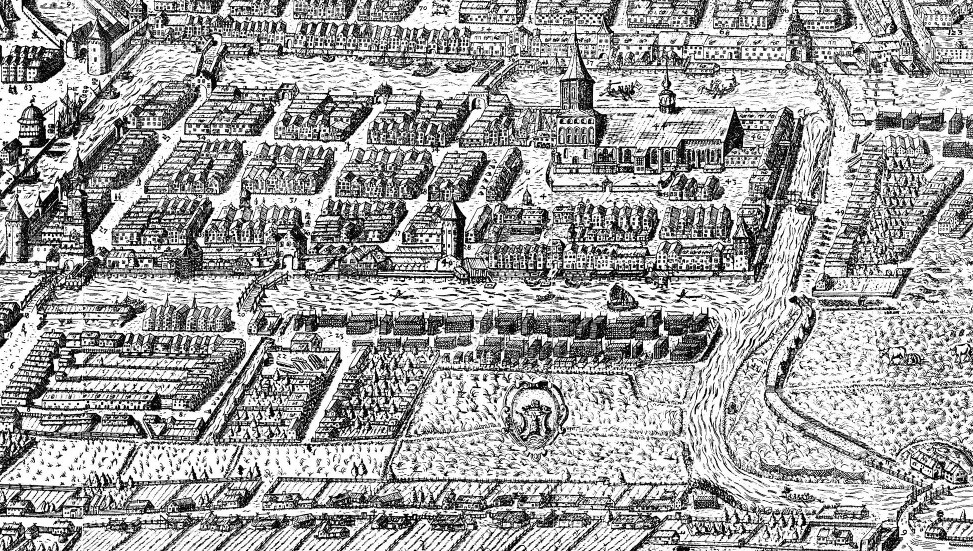
\includegraphics[width=\textwidth]{Koenigsberg}
    \caption{%
      A map of Königsberg from about 1813. Modified from an engraving by
      Joachim Bering from 1613. For annotations, you could use
      \texttt{TikZ} or the \texttt{overpic} package.
    }
    \label{fig:Koenigsberg}
  \end{figure}
\end{verbatim}
%
Figure~\autoref{fig:Koenigsberg} on~\pageref{fig:Koenigsberg} depicts an
example.
%
Please ensure that figures are referenced properly and give credit to
the original author if you use a figure from a publication.
%
You should also check that the resolution of the figure is sufficient.
%
If in doubt, recreate the figure yourself, using \verb|TikZ|\footnote{\url{http://www.texample.net/tikz}}, \verb|pgfplots|\footnote{\url{http://pgfplots.sourceforge.net}}, or any vector graphics application such as \verb|Inkscape|\footnote{\url{https://inkscape.org/en}}.

\begin{figure}[t]
  \centering
  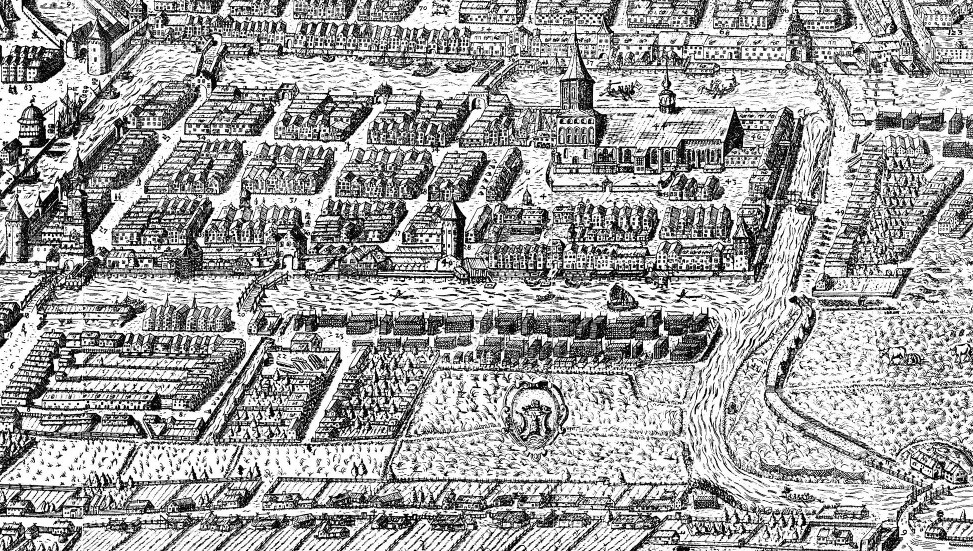
\includegraphics[width=\textwidth]{Koenigsberg}
  \caption{%
    A map of Königsberg from about 1813. Modified from an engraving by
    Joachim Bering from 1613. For annotations, you could use
    \texttt{TikZ} or the \texttt{overpic} package.
  }
  \label{fig:Koenigsberg}
\end{figure}

If you want to add multiple subordinate figures under a larger figure,
use the \verb|subcaption| package that is included by default. It is
good practice to use the \verb|\subcaptionbox| command for wrapping
figures. The first parameter to this command is the caption of the
figure. It may remain empty or contain only a \verb|\label| command for
subsequent references. It is possible to refer to the complete
sub-figure using the usual reference commands. If you want to refer to
an individual sub-figure only, use the \verb|\subref| command.
%
\begin{verbatim}
  \begin{figure}
    \centering
    \subcaptionbox{Label\label{sfig:Label}}{%
      \begin{tikzpicture}
        ...
      \end{tikzpicture}
    }
  \end{figure}
\end{verbatim}
%
\autoref{fig:Anscombe's quartet} depicts numerous sub-figures in order
to show all members of Anscombe's quartet. \autoref{sfig:Anscombe's
quartet A} is the first one of these. This figure is also denoted
by~\subref{sfig:Anscombe's quartet A}, although you should use such
a reference only within a caption because it may be confusing to
readers---and by extension, it may also confuse the people who grade
your report.

Please refer to the source code for more information. It also
demonstrates the use of the \verb|pgfplots| package for high-quality
typesetting of statistical graphics. An introduction would go beyond the
scope of this document, though, but this package is highly recommend if
you want your graphics to have a consistent look-and-feel. 

\begin{figure}
  \centering
  \pgfplotsset{%
    Anscombe/.style={%
      axis x line   = bottom,
      axis y line   = left,
      %
      only marks,
      %
      enlargelimits = false,
      xmin          =  3.5,
      xmax          = 20.0,
      ymin          =  4.0,
      ymax          = 13.0,
      %
      width         = 0.5\linewidth,
      height        = 4cm,
    }
  }
  \subcaptionbox{\label{sfig:Anscombe's quartet A}}{%
    \begin{tikzpicture}
      \begin{axis}[Anscombe]
        \addplot[black, mark=*] table {Data/Anscombe_1.txt};
        \addplot[sharp plot, domain={\pgfplotsxmin:\pgfplotsxmax}] { 3 + 0.5*x };
      \end{axis}
    \end{tikzpicture}
  }
  \subcaptionbox{}{%
    \begin{tikzpicture}
      \begin{axis}[Anscombe]
        \addplot[black, mark=*] table {Data/Anscombe_2.txt};
        \addplot[sharp plot, domain={\pgfplotsxmin:\pgfplotsxmax}] { 3 + 0.5*x };
      \end{axis}
    \end{tikzpicture}
  }\\
  \subcaptionbox{}{%
    \begin{tikzpicture}
      \begin{axis}[Anscombe]
        \addplot[black, mark=*] table {Data/Anscombe_3.txt};
        \addplot[sharp plot, domain={\pgfplotsxmin:\pgfplotsxmax}] { 3 + 0.5*x };
      \end{axis}
    \end{tikzpicture}
  }
  \subcaptionbox{}{%
    \begin{tikzpicture}
      \begin{axis}[Anscombe]
        \addplot[black, mark=*] table {Data/Anscombe_4.txt};
        \addplot[sharp plot, domain={\pgfplotsxmin:\pgfplotsxmax}] { 3 + 0.5*x };
      \end{axis}
    \end{tikzpicture}
  }
  \caption{%
    Multiple figures are best shown using the \texttt{subcaption}
    package. Individual figures may be referenced using the
    \texttt{\textbackslash{}subref} command.
    %
    \subref{sfig:Anscombe's quartet A} depicts the first member of Anscombe's
    quartet, a classical data set in statistics.
  }
  \label{fig:Anscombe's quartet}
\end{figure}

\subsection{Typesetting mathematics}

This template uses \verb|amsmath| and \verb|amssymb|, which are the
de-facto standard for typesetting mathematics. Use numbered equations
using the \verb|equation| environment.
%
If you want to show multiple equations and align them, use the
\verb|align| environment:
%
\begin{align}
    V &:= \{ 1, 2, \dots \}\\
    E &:= \big\{ \left(u,v\right) \mid \dist\left(p_u, p_v\right) \leq \epsilon \big\}
\end{align}
%
Define new mathematical operators using \verb|\DeclareMathOperator|. See
the template for some examples. Else, your operator will be typeset
incorrectly. Observe the difference between the incorrect~(left) and
correct~(right) usage: 
%
\begin{equation}
  cos x \neq \cos x
\end{equation}
%
Moreover, this template contains a correct differential operator. Use \verb|\d| to typeset the differential of integrals:
%
\begin{equation}
  f(u) := \int_{v \in \mathds{D}}\dist(u,v)\d{v}
\end{equation}
%
Take a look at the source for more examples. If in doubt, ask the
organizers for help.

The documentation of the \verb|amsmath|
package\footnote{\url{http://mirrors.ctan.org/macros/latex/required/amsmath/amsmath.pdf}}
is also extremely useful.
%
Likewise, the guide by Mark
Tomforde\footnote{\url{https://www.math.uh.edu/~tomforde/MathWriting.pdf}}
contains a variety of useful tips and tricks.
%
Remember that typesetting complicated things takes some time, but is
usually worth the effort because \emph{you} understand it better, and so
the reader might understand it better as well.

\subsection{Typesetting algorithms}

This template suggests using the \verb|algorithmi| package for
typesetting an algorithm.
%
It is customizable and offers sufficient flexibility to cover most usage scenarios. Feel free to use another package, though, or refer to the extensive documentation\footnote{\url{http://mirror.unl.edu/ctan/macros/latex/contrib/algorithmicx/algorithmicx.pdf}}.
%
There's no standard for pseudo-code, so feel free to use any format that
seems acceptable to you. Always use a caption and a label for your algorithm, so that you may refer to it correctly, e.g.\ \autoref{alg:Persistent homology}.

Notice that for most reports, adding specific algorithms should not be
necessary. However, you are free to go the extra mile if you consider
this to improve the report, in particular if you reference the algorithm
numerous times or if the implementation is a large part of the
contribution.

\begin{algorithm}[t]
  \caption{0-dimensional persistent homology calculation}
  \label{alg:Persistent homology}
  %
  \begin{algorithmic}[1]
    \newcommand{\UF}{\texttt{UF}}
    \newcommand{\diagram}{\mathcal{D}}
    \newcommand{\graph}  {\mathcal{G}}
    \newcommand{\weight} {\mathrm{w}}
    %
    \Require A weighted graph $\graph$
    \State $\UF \gets \emptyset$\Comment{Initialize an empty Union--Find structure}
    \State $\diagram \gets \emptyset$\Comment{Initialize an empty persistence diagram}
    \For{every edge $(u,v)\in\graph$ in ascending order of its weight}
      \State $c \gets$  $\UF$\texttt{.Find}($u$)
      \State $c' \gets$ $\UF$\texttt{.Find}($v$)
      \If{$\weight(c) < \weight(c')$}\Comment{$c$ is the older component; merge $c'$ into it}
        \State $\UF$\texttt{.Union}($c'$, $c$)
        \State $\diagram\gets\diagram\cup\big(\weight(c'), \weight(u,v)\big)$
      \Else\Comment{$c'$ is the older component; merge $c$ into it}
        \State $\UF$\texttt{.Union}($c$, $c'$)
        \State $\diagram\gets\diagram\cup\big(\weight(c) , \weight(u,v)\big)$
      \EndIf
    \EndFor
    \State\Return$\diagram$
  \end{algorithmic}
\end{algorithm}
